\chapter{To The Motif Finding Problem}\label{motiffindingproblem}
Our target is to identify a motif from a DNA sequence. In our study
we only deal with transcription factor binding sites. We will give
the formal definition of the motif finding problem later. Assume
that we are given some DNA sequence of nucleotides which are generated
randomly. Now, we want to find a secret pattern that occurs at least
one time in every given DNA sequence without any prior knowledge
about how it looks like. This pattern is our motif.

Some complications encountered while finding motifs:
\begin{itemize}
	\item We do not know the motif sequence.
	\item Hence we donot know what to search for in the DNA sequence.
	\item We do not know where the motifs are located relative to
	the starting index of the sequence.
	\item Motifs can differ in one or more positions in their
	sequence which is called mutations.
	\item How to discern functional motifs from random ones?
	
\end{itemize}

The idea is illustrated in the \Cref{fig:seq1}, \Cref{fig:seq2}
and \Cref{fig:seq2}.

\begin{figure}%[!tb]
	\centering
	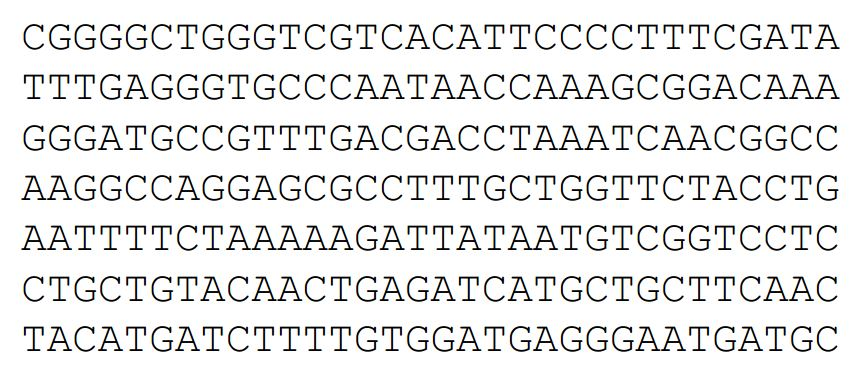
\includegraphics[width=0.6\textwidth]{figures/seq1}
	\caption{Seven random sequences.}
	\label{fig:seq1}
\end{figure}
\begin{figure}[!tb]
	\centering
	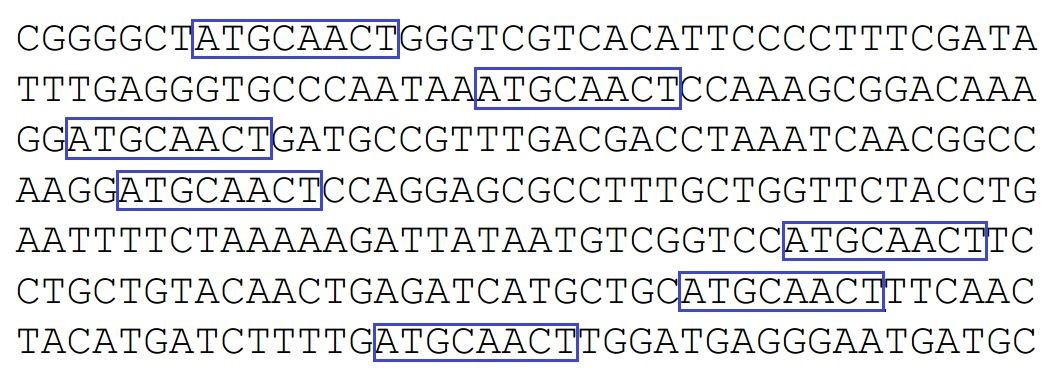
\includegraphics[width=0.75\textwidth]{figures/seq2}
	\caption{The same DNA sequences of \Cref{fig:seq1}
		with the implanted pattern ATGCAACT.}
	\label{fig:seq2}
\end{figure}
\begin{figure}[!tb]
	\centering
	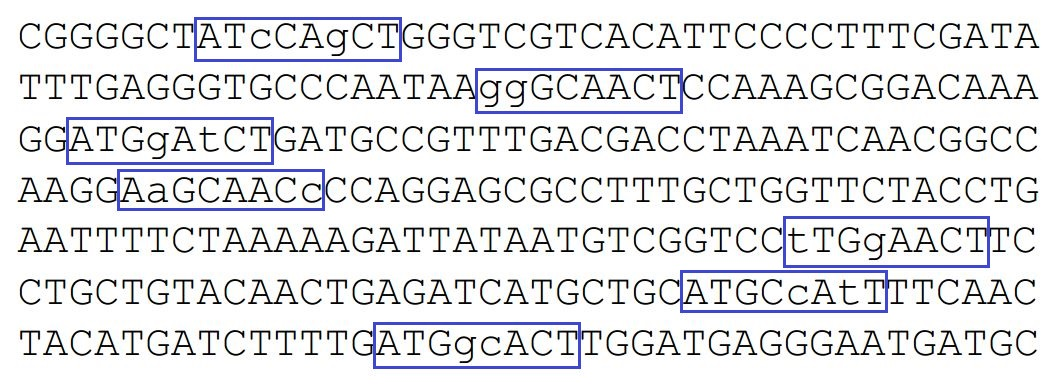
\includegraphics[width=0.75\textwidth]{figures/seq3}
	\caption{Same as \Cref{fig:seq2} with the implanted
		pattern ATGCAACT randomly
		mutated in two positions.}
	\label{fig:seq3}
\end{figure}


\section{Alignment Matrix}
To formulate the motif finding problem we first need to define
what we mean by motif. As we saw in \Cref{fig:seq3} there may be
mismatch in some positions of the motifs.

\begin{figure}%[!tb]
	\centering
	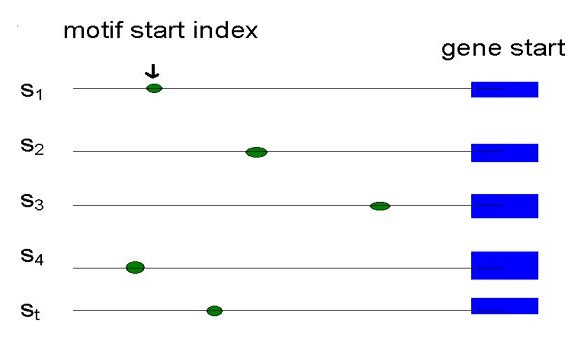
\includegraphics[width=0.6\textwidth]{figures/sindex}
	\caption{Starting index of motifs in a DNA sequence .}
	\label{fig:sindex}
\end{figure}


Now consider a set of \textit{t} DNA sequences $ S_{1}, S_{2},\ldots,
S_{t} $. Each of which has \textit{n} nucleotides. We select one
position in each of these \textit{t} sequences, thus forming an array
$ s = (s_{1}, s_{2},\ldots,s_{t}) $, where $ 1 \leq s_{i} \leq n - l + 1$
\Cref{fig:sindex}.
Here \textit{l} is the length of the pattern. The superposition
of the \textit{l}-mers of \Cref{fig:seq3} is shown in \Cref{fig:superpose}.
Now taking the \textit{l}-mers starting at these positions
we can compile a \textit{alignment matrix}\index{Alignment Matrix}
of $ t × l $. The $ (i, j) $th element of the \textit{alignment matrix}
is the nucleotide at the $ s_{i} + j − 1 $th position in the
\textit{i}th sequence. Illustrations are shown in \Cref{fig:consensus}.


\begin{figure}%[!tb]
	\centering
	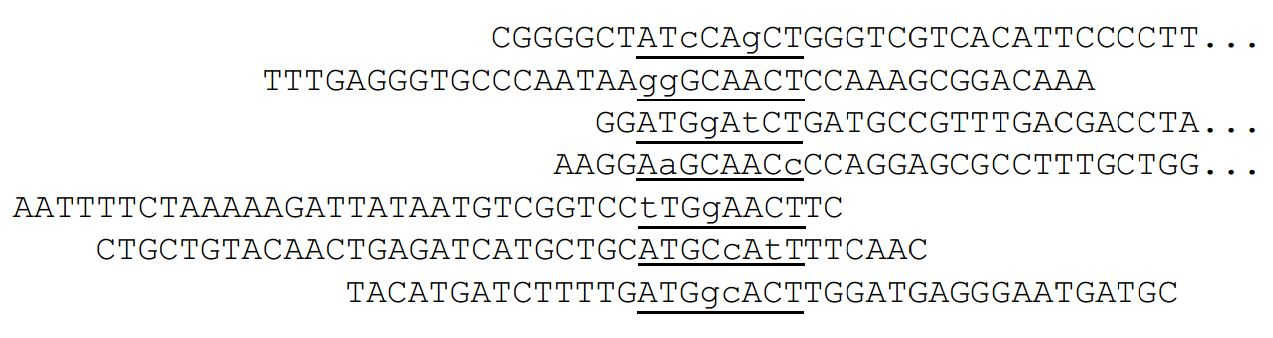
\includegraphics[width=1.0\textwidth]{figures/superpose}
	\caption{Superposition of the seven highlighted 8-mers from \Cref{fig:seq2}.}
	\label{fig:superpose}
\end{figure}
\begin{figure}%[!tb]
	\centering
	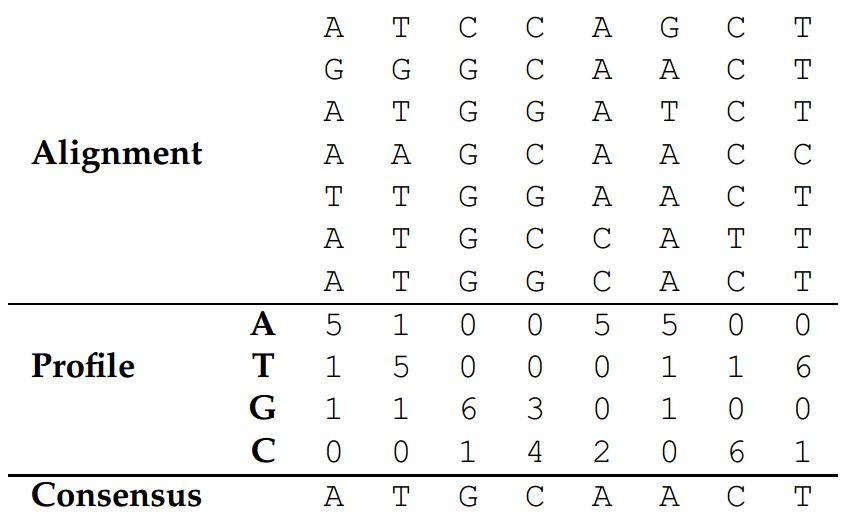
\includegraphics[width=0.7\textwidth]{figures/consensus}
	\caption{The alignment matrix, profile matrix and consensus
		string formed from the 8-mers starting at positions
		$ s = (8, 19, 3, 5, 31, 27, 15) $ in \Cref{fig:seq2}.}
	\label{fig:consensus}
\end{figure}



\section{Profile Matrix}
The \textit{profile matrix}\index{Profile Matrix} or profile, illustrates
the variability of nucleotide composition at each position for
a particular group of \textit{l}-mers. Let the alphabet $ \Sigma $
in our motif search. Then the size of the \textit{profile matrix} will be
$ | \Sigma | \times l$. For DNA $ | \Sigma | = 4$.  Based on the
\textit{alignment matrix}, we can compute the $ 4 \times l $
\textit{profile matrix} whose $ (i, j) $th element holds the
number of times nucleotide $ i $ appears in column
$ j $ of the \textit{alignment matrix}, where $ i $ varies from 1 to 4.
In \Cref{fig:consensus} we see that positions 3, 7, and
8 are highly conserved, while position 4 is not.


\section{Consensus String}
To further summarize the profile matrix, we can form a consensus string from the most popular element in each column of the alignment matrix. It is the nucleotide with the largest entry in the profile matrix. \Cref{fig:consensus} shows the alignment matrix for s = (8,19,3,5,31,27,15), the corresponding profile matrix, and the resulting
consensus string ATGCAACT.

\section{Evaluating Motifs}
By varying the starting positions in s, we can construct a large number of
different profile matrices from a given sample. Some profiles represent high conservation of a pattern while others represent no conservation at all. An imprecise formulation of the Motif Finding problem is to find the starting positions s corresponding to the most conserved profile. 

\subsection{Scoring Function}
If $ P(s) $ denotes the profile matrix corresponding to starting positions s, then
we will use $ M_{P(s)}(j) $ to denote the largest count in column j of $ P(s) $. For
the profile P(s) in \Cref{fig:consensus}, $ M_{P(s)}(1) = 5, M_{P(s)}(2) = 5$ , and  $ M_{P(s)}(8) = 6 $.
Given starting positions s, the consensus score is defined to be $ Score(s, DNA) =
\sum_{j=1}^{l}M_{P(s)}(j) $. In our case, $ Score(s, DNA) =
5 + 5 + 6 + 4 + 5 + 5 + 6 + 6 = 42 $. $  Score(s, DNA) $ can be used to measure the strength of a profile corresponding to the starting positions s.


\section{Defining The Motif Finding Problem}
the Motif Finding problem can be formulated as selecting starting positions s from the sample that maximize $ Score(s, DNA) $. 
\begin{table}[H]
	\begin{center}
		\begin{tabular}{p{300 pt}}
			\hline
			\textbf{Motif Finding Problem:}\\
			\textit{Given a set of DNA sequences, find a set of l-mers, one from each
			sequence, that maximizes the consensus score.}\\
		
			\textbf{Input:} A t×n matrix of DNA, and l, the length of the pattern
			to find.\\
			
			\textbf{Output:} An array of t starting positions s = (s1, s2, . . . , st)
			maximizing Score(s, DNA).\\
			\hline
		\end{tabular}
	\end{center}
\end{table}

\endinput